\documentclass{beamer}

%gets rid of bottom navigation bars
\setbeamertemplate{footline}[page number]{}

%gets rid of navigation symbols
\setbeamertemplate{navigation symbols}{}

\title{Single-cell RNA sequencing for beginners}

\author{Aaron Lun \\[0.1in]
\footnotesize{CRUK Cambridge Institute}
}

\date{
\footnotesize{Tel Aviv University}\\[0.1in]
23 May 2018
}


\makeatletter
\newlength\beamerleftmargin
\setlength\beamerleftmargin{\Gm@lmargin}
\makeatother

\begin{document}
\maketitle

\begin{frame}{Why do single-cell RNA sequencing?}

\begin{exampleblock}{Why single cells?}
A lot of biology occurs at the cellular level:
\begin{itemize}
\item Cell identity (e.g., cell types)
\item Cell behaviour and status (e.g., stress, metabolism, cell cycle)
\item Cellular dynamics (differentiation, activation)
\end{itemize}
\end{exampleblock}

\begin{exampleblock}{Why RNA sequencing?}
Quantify expression of every gene\footnote{poly A'd} in the transcriptome:
\begin{itemize}
\item FACS: small number of proteins
\item FISH: small number of transcripts
\end{itemize}
\end{exampleblock}
\end{frame}

\begin{frame}{A ``typical'' scRNA-seq protocol}
\noindent\makebox[\textwidth]{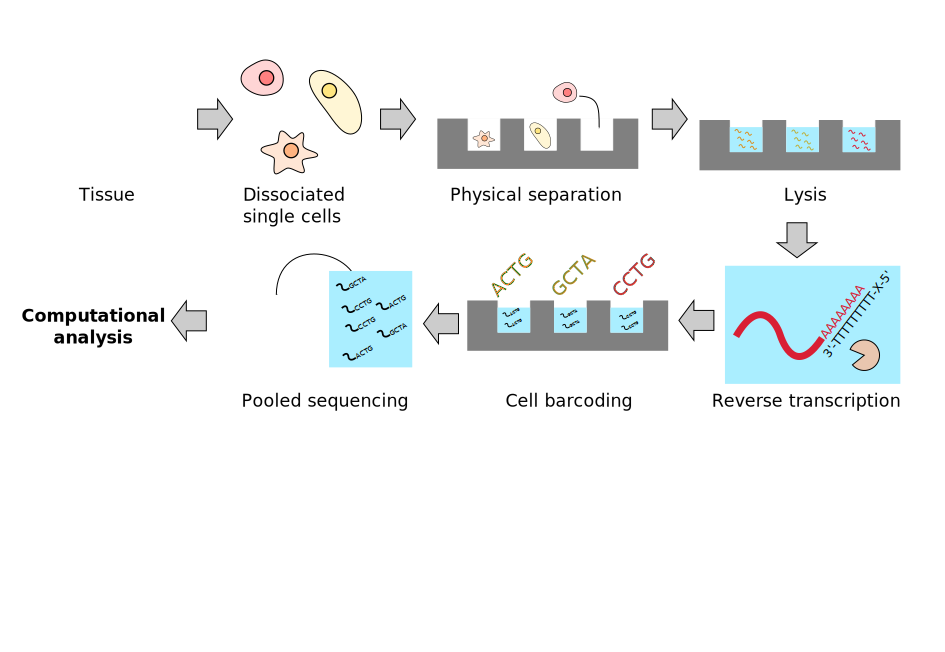
\includegraphics[width=0.95\paperwidth]{pics/overview.pdf}}\\[0.1in]

\begin{itemize}
\item Dissociation can be easy (blood) or hard (muscle).
\item Protocols differ in how they perform separation and RT.
\end{itemize}
\end{frame}

\begin{frame}{Physical separation methods: microfluidics}
Most popular of which is the Fluidigm C1 (96 cells per chip):
\begin{center}
\includegraphics[width=0.7\textwidth]{pics/fluidigm_c1.jpg}
\end{center}
Less common nowadays due to cost, throughput, doublet issues
\end{frame}

\begin{frame}{Physical separation methods: cell sorting}
Sort individual cells into 96/384-well plates (``plate-based''):

\begin{center}
\includegraphics[width=0.5\textwidth]{pics/facs_to_plate.pdf}
\end{center}

Cheap, provides extra phenotypic data, easy to customize:\\
$\quad\hookrightarrow$ control wells, spike-ins, randomization, automation
\end{frame}

\begin{frame}{Physical separation methods: droplets}
Capture cells in aqueous droplets in oil suspension (e.g., 10X):

\begin{center}
\includegraphics[width=0.65\textwidth]{pics/droplets.pdf}
\end{center}

Very high throughput (4000-10000 per run) but noisier per cell.
\end{frame}

\begin{frame}{cDNA library prep: protocol overview}
Most\footnote{All?} protocols use oligo-dT primers for first-strand synthesis.
\begin{center}
\includegraphics[width=0.8\textwidth,trim=0mm 45mm 0mm 0mm,clip]{pics/grun_design.jpg} \\
{\tiny Adapted from Gr\"un and van Oudenaarden, 2015, \emph{Cell}.}
\end{center}
\end{frame}

\begin{frame}{cDNA library prep: unique molecular identifiers}
\begin{center}
\includegraphics[width=0.8\textwidth]{pics/umis.pdf}
\end{center}

Dedupping with UMIs to reduce amplification noise (5'/3' biased)\\
$\quad\hookrightarrow$ CEL-seq2, STRT-seq, droplet-based methods
\end{frame}

\begin{frame}{Cell barcoding: the motivation}
Modern Illumina sequencers have massive throughput:
\begin{itemize}
\item $> 3 \times 10^8$ reads per lane 
\item 8 lanes per flow cell
\item 2 flow cells per run (HiSeq 4000)
\end{itemize}
\pause
\begin{exampleblock}{Multiplexing - what and why?}
Pool cDNA from many cells together, and sequence the pool.
\begin{itemize}
\item More cost-effective - spread coverage across cells
\item Logistically easier - robust to lane failures
\end{itemize}
\end{exampleblock}
\pause
Deumultiplexing = assigning pooled reads back to cell of origin
\begin{itemize}
\item Label cDNA from each cell with a unique sequence (``barcode'') prior to pooling
\item Identify barcode from sequenced reads
\end{itemize}
\end{frame}

\begin{frame}{Cell barcoding: strategies}
Cell barcode in the PCR primer:
\begin{itemize}
\item incorporated into the amplicon upon extension 
\item plate-based only; add different primers to each well
\end{itemize}
Cell barcode in the oligo-dT primer:
\begin{center}
\includegraphics[width=0.9\textwidth]{pics/barcodes.pdf}
\end{center}
\end{frame}

\begin{frame}{Brief overview of reversible terminator sequencing}
\begin{minipage}{0.69\textwidth}
\includegraphics[width=0.9\textwidth,trim=0mm 80mm 140mm 5mm,clip]{pics/sequencing_metzker.jpg} 
\end{minipage}
\begin{minipage}{0.29\textwidth}
{\tiny Adapted from Metzker, 2010, \\\textit{Nature Reviews Genetics}}
\end{minipage}
\end{frame}

\begin{frame}{Sequencing data formats: FASTQ}
\begin{enumerate}
\item Read name, starting with \texttt{@}
\item Read sequence, usually of constant length from 50-150 bp
\item \texttt{+} separator
\item Read quality, encoded as ASCII + 33 {\tiny (Quality of 40 $\to$ 40 + 33 $\to$ 73 $\to$ \texttt{I})}
\end{enumerate}
\begin{center}
\includegraphics[width=\textwidth,trim=0mm 84mm 150mm 0mm,clip]{pics/fastq.png}
\end{center}
Paired-end data has 2 FASTQs per library (10X data has 3!)\\
$\quad\hookrightarrow$ paired reads have the same name      
\end{frame}

\begin{frame}{Sequencing data formats: SAM/BAM}
\textbf{Align} reads to a reference genome (or transcriptome).
\begin{itemize}
\item Read sequences ``mapped'' to originating location.
\item Can be tricky for intron-spanning reads, repeat regions!
\item Many good \& fast aligners - \texttt{subread}, \texttt{STAR}, etc.
\end{itemize}
\vspace{0.1in}
\textbf{S}equence \textbf{A}lignment/\textbf{M}ap format (BAM = compressed)
\begin{center}
\includegraphics[width=\textwidth]{pics/sam.png}
\end{center}
Stores alignment information for each read.
\end{frame}

\begin{frame}{Quantifying gene expression per cell}
Count the number of reads mapping to exonic regions of each gene:
\begin{center}
\includegraphics[width=\textwidth]{pics/feature_counts.pdf}
\end{center}
\begin{itemize}
\item Handling paired reads, exon-exon reads, overlapping genes?
\item Collapsing reads with the same UMI into a single count
\item Pseudo-aligners, e.g., \texttt{salmon}, \texttt{kallisto}
\end{itemize}
\vspace{0.1in}
\textbf{Endpoint:} one read (or UMI) count per gene per cell
\end{frame}

\begin{frame}{What does scRNA-seq data look like?}
A typical scRNA-seq count matrix:
\begin{center}
\includegraphics[width=\textwidth]{../computational/pics/scData.pdf} \\
\vspace{-.1in}
{\tiny Data from \textit{Science} (2015), 347:1138-42}
\end{center}
\begin{itemize}
\item lots of zeros due to dropout events (\textbf{or no expression!})
\item variable total counts across cells - cell-specific biases
\item variable counts per gene - part biological, part technical
\end{itemize}
\end{frame}

\begin{frame}{Single-cell data analysis}
\textbf{Aim:} To extract real biology from data with technical noise
\begin{enumerate}
\item Quality control
\item Normalization 
\item Batch correction
\item Dimensionality reduction and visualization
\item Clustering
\end{enumerate}
\end{frame}

\begin{frame}{Quality control on the cells}
Remove low quality cells:
\begin{itemize}
\item Low total counts (``library size'') 
\item Low number of expressed genes (non-zero counts) 
\item High percentage of spike-in or mitochondrial reads 
\end{itemize}
\pause
\begin{center}
\includegraphics[width=0.9\textwidth]{pics/cell_damage.pdf}
\end{center}
\end{frame}

\begin{frame}{Distributions of spike-in, mitochondrial proportions}
Various batches of human ESCs:
\begin{center}
\includegraphics[width=\textwidth]{../computational/pics/mitoAndSpikes_WR.png}
\end{center}
{\tiny Data from Ferdinand von Meyenn and Wolf Reik at the Babraham Institute}
\end{frame}


\begin{frame}{Normalization for cell-specific biases}
Differences in library size, capture efficiency, composition bias:
\begin{center}
\includegraphics[width=0.7\textwidth]{pics/cell_biases.pdf}
\end{center}
\end{frame}

\begin{frame}{Scaling normalization}
Scaling normalization to remove biases \textit{between} cells \\
$\quad\hookrightarrow$ compute a ``size factor'' to divide the counts for each cell \\[0.1in]
\textbf{To demonstrate:} consider counts for a few genes in a few cells
\begin{itemize}
\item assume X, Y, Z... are \textit{not} DE between cells
\item systematic fold-differences are technical in origin
\end{itemize}

\begin{center}
\begin{tabular}{l p{0.2in} p{0.2in} p{0.2in} p{0.2in}}
\hline
\textbf{Cell} & \textbf{A} & \textbf{B} & \textbf{C} & \textbf{D} \\
\hline
Gene X & 10 & \alt<1>{20}{\textcolor{red}{10}} & \alt<1>{30}{\textcolor{red}{10}} & \alt<1>{40}{\textcolor{red}{10}} \\
Gene Y & 15 & \alt<1>{30}{\textcolor{red}{15}} & \alt<1>{45}{\textcolor{red}{15}} & \alt<1>{60}{\textcolor{red}{15}} \\
Gene Z & 20 & \alt<1>{40}{\textcolor{red}{20}} & \alt<1>{60}{\textcolor{red}{20}} & \alt<1>{80}{\textcolor{red}{20}} \\
& ... & ... & ... & ... \\ 
\hline
\textbf{Size factor} & 1 & 2 & 3 & 4 \\
\hline
\end{tabular}
\end{center}
\pause
Scales \textit{down} counts prior to comparisons between cells 
\end{frame}

\begin{frame}{Normalization and composition biases}
\begin{center}
\includegraphics[width=\textwidth]{pics/composition_bias.pdf}
\end{center}
Composition biases introduced by differential expression:
\begin{itemize}
\item Competition for the ``sequencing pie''
\item Normalization by library size is particularly susceptible
\item Requires methods robust to DE
\end{itemize}
\end{frame}

\begin{frame}{Normalization in real data}
Up to and over an order of magnitude difference in scaling:
\begin{center}
\includegraphics[width=0.45\textwidth]{pics/416B_LibvDeconv.png}\vspace{0.1in}
\includegraphics[width=0.45\textwidth]{pics/zeisel_LibvDeconv.png}
\end{center}
\begin{itemize}
\item[Left:] 416B cells with oncogene induction {\tiny (Lun et al., 2017, \textit{Genome Research})}
\item[Right:] Mouse brain cells {\tiny (Zeisel et al., 2015, \textit{Science})}
\end{itemize}
\end{frame}

\begin{frame}{Dimensionality reduction with PCA}
PCA = principal components analysis
\begin{itemize}
\item identifies axes of maximal variance in high-dimensional data
\item each principal component (PC) explains less variance 
\end{itemize}
\begin{center}
\includegraphics[width=\textwidth,trim=0mm 5mm 0mm 40mm,clip]{../computational/pics/pca_explanation.pdf}
\end{center}
\textbf{Use the first few (5-100) PCs as a ``summary'' of the data}
\begin{itemize}
\item Speed up downstream analyses by reducing dimensionality
\item Focus on biology, remove random noise in later PCs
\end{itemize}
\vspace{0.1in}
Alternative to using top HVGs for clustering, $t$-SNE, etc.
\end{frame}

\begin{frame}{Visualization with PCA}
The first 2-3 PCs can be directly used for visualization:
\begin{center}
\includegraphics[width=0.9\textwidth]{../computational/pics/pca_brain_SL.png} \\
    {\tiny Data from Zeisel et al., 2015, \textit{Science}}
\end{center}
Simple and efficient, but limited resolution of complex structure.
% Internal differences within blobs not visible, dominated by differences between blobs.
\end{frame}

\begin{frame}{Visualization with $t$-SNE}
Finds a low-dimensional representation of high-dimensional data 
\begin{itemize}
    \item preserve distances to neighbouring cells
    \item non-linear: not limited to straight axes
\end{itemize}
\begin{center}
    \includegraphics[width=0.9\textwidth]{../computational/pics/tsne_brain_SL.png} \\
    {\tiny Data from Zeisel et al., 2015, \textit{Science}}
\end{center}
Powerful, but need to fiddle with random seed and perplexity
\end{frame}

\begin{frame}{Batch correction}
Large datasets need to be processed in multiple batches: 
\begin{itemize}
\item Batch effects caused by differences in processing
\item Correction based on common subpopulations
\end{itemize}
\vspace{0.1in}
\begin{minipage}{0.49\textwidth}
\begin{flushleft}
\textbf{Before correction}
\includegraphics[width=\textwidth]{pics/haem_raw.png} \\
\end{flushleft}
\end{minipage}
\begin{minipage}{0.49\textwidth}
\begin{flushleft}
\textbf{After correction}
\includegraphics[width=\textwidth]{pics/haem_corrected.png} \\
\end{flushleft}
\end{minipage}
\\[0.1in]
{\tiny Data from Nestorawa et al., 2016, \textit{Blood}; Paul et al., 2015, \textit{Cell}}
\end{frame}

\begin{frame}{Clustering strategies}
Group cells with similar expression profiles into ``clusters'': 
\begin{itemize}
\item annotate as particular cell types or states
\item interpretable summary of the data
\end{itemize}
\vspace{0.1in}
Definition of a cluster depends on the method:
\begin{center}
\includegraphics[width=\textwidth]{pics/clustering.pdf}
\end{center}
\end{frame}

\begin{frame}{Real applications: pluripotency}
Identify new hESC population between naive/primed cells:
\begin{center}
\includegraphics[width=0.49\textwidth, trim=0mm 0mm 0mm 20mm,clip]{pics/hESC_transition.pdf}
\includegraphics[width=0.49\textwidth, trim=0mm 0mm 0mm 0mm,clip]{pics/hESC_heatmap.pdf}\\
{\tiny von Meyenn et al., 2018, in prep.}
\end{center}
\end{frame}

\begin{frame}{Real applications: ageing}
CD4$^+$ T cells become more variable with age: 
\begin{center}
\includegraphics[width=\textwidth,trim=0mm 50mm 0mm 0mm,clip]{pics/tcell_aging.jpg} \\
{\tiny Martinez-Jimenez et al., 2017, \textit{Science}}
\end{center}
\end{frame}

\begin{frame}{Real applications: embryonic development}
\begin{center}
\includegraphics[width=0.75\textwidth]{pics/gastrulation.jpg} \\
{\tiny Ibarra-Soria et al., 2018, \textit{Nature Cell Biology}}
\end{center}
\end{frame}

\begin{frame}{Wrapping up}
Experimental protocols:
\begin{itemize}
\item How are cells separated and barcoded?
\item With or without UMIs?
\end{itemize}

Computational methods for data analysis:
\begin{itemize}
\item separate technical effects from real biology:
\item quality control, normalization, batch correction, etc.
\end{itemize}
\vspace{0.1in}
\begin{center}
\includegraphics[height=0.5in]{../computational/pics/cruk_logo.png} \hspace{0.1in}
\includegraphics[height=0.5in]{../computational/pics/cam_logo.jpg} 
\end{center}
\end{frame}

\end{document}
